%% LyX 2.3.4.2 created this file.  For more info, see http://www.lyx.org/.
%% Do not edit unless you really know what you are doing.
\documentclass[english,dvipsnames,aspectratio=169,handout]{beamer}
\usepackage{mathptmx}
\usepackage{eulervm}
\usepackage[T1]{fontenc}
\usepackage[latin9]{inputenc}
\usepackage{babel}
\usepackage{amstext}
\usepackage{amssymb}
\usepackage{graphicx}
\usepackage{ifthen}
\usepackage{xcolor}
\usepackage{xspace}
\usepackage{tikz}
\usetikzlibrary{tikzmark}
\usetikzlibrary{calc}
\usepackage{pgfplots}
%\pgfplotsset{compat=1.17}
\usepackage{booktabs}
\usepackage{xpatch}
\usepackage{multirow}
\usepackage{colortbl}
\usepackage{pgfpages}


\xpatchcmd{\itemize}
  {\def\makelabel}
  {\ifnum\@itemdepth=1\relax
     \setlength\itemsep{2ex}% separation for first level
   \else
     \ifnum\@itemdepth=2\relax
       \setlength\itemsep{1ex}% separation for second level
     \else
       \ifnum\@itemdepth=3\relax
         \setlength\itemsep{0.5ex}% separation for third level
   \fi\fi\fi\def\makelabel
  }
 {}
 {}

\ifx\hypersetup\undefined
  \AtBeginDocument{%
    \hypersetup{unicode=true,pdfusetitle,
 bookmarks=true,bookmarksnumbered=false,bookmarksopen=false,
 breaklinks=false,pdfborder={0 0 0},pdfborderstyle={},backref=false,colorlinks=true,
 allcolors=NYUPurple,urlcolor=LightPurple}
  }
\else
  \hypersetup{unicode=true,pdfusetitle,
 bookmarks=true,bookmarksnumbered=false,bookmarksopen=false,
 breaklinks=false,pdfborder={0 0 0},pdfborderstyle={},backref=false,colorlinks=true,
 allcolors=NYUPurple,urlcolor=LightPurple}
\fi

\makeatletter

%%%%%%%%%%%%%%%%%%%%%%%%%%%%%% LyX specific LaTeX commands.
%% Because html converters don't know tabularnewline
\providecommand{\tabularnewline}{\\}

%%%%%%%%%%%%%%%%%%%%%%%%%%%%%% Textclass specific LaTeX commands.
% this default might be overridden by plain title style
\newcommand\makebeamertitle{\frame{\maketitle}}%
% (ERT) argument for the TOC
\AtBeginDocument{%
  \let\origtableofcontents=\tableofcontents
  \def\tableofcontents{\@ifnextchar[{\origtableofcontents}{\gobbletableofcontents}}
  \def\gobbletableofcontents#1{\origtableofcontents}
}

%%%%%%%%%%%%%%%%%%%%%%%%%%%%%% User specified LaTeX commands.
\usetheme{CambridgeUS} 
\beamertemplatenavigationsymbolsempty


% Set Color ==============================
\definecolor{NYUPurple}{RGB}{87,6,140}
\definecolor{LightPurple}{RGB}{165,11,255}


\setbeamercolor{title}{fg=NYUPurple}
\setbeamercolor{frametitle}{fg=NYUPurple}

\setbeamercolor{background canvas}{fg=NYUPurple, bg=white}
\setbeamercolor{background}{fg=black, bg=NYUPurple}

\setbeamercolor{palette primary}{fg=black, bg=gray!30!white}
\setbeamercolor{palette secondary}{fg=black, bg=gray!20!white}
\setbeamercolor{palette tertiary}{fg=gray!20!white, bg=NYUPurple}

\setbeamertemplate{headline}{}
\setbeamerfont{itemize/enumerate body}{}
\setbeamerfont{itemize/enumerate subbody}{size=\normalsize}

\setbeamercolor{parttitle}{fg=NYUPurple}
\setbeamercolor{sectiontitle}{fg=NYUPurple}
\setbeamercolor{sectionname}{fg=NYUPurple}
\setbeamercolor{section page}{fg=NYUPurple}
%\setbeamercolor{description item}{fg=NYUPurple}
%\setbeamercolor{block title}{fg=NYUPurple}

\setbeamertemplate{blocks}[rounded][shadow=false]
\setbeamercolor{block body}{bg=normal text.bg!90!NYUPurple}
\setbeamercolor{block title}{bg=NYUPurple!30, fg=NYUPurple}



\AtBeginSection[]{
  \begin{frame}
  \vfill
  \centering
\setbeamercolor{section title}{fg=NYUPurple}
 \begin{beamercolorbox}[sep=8pt,center,shadow=true,rounded=true]{title}
    \usebeamerfont{title}\usebeamercolor[fg]{title}\insertsectionhead\par%
  \end{beamercolorbox}
  \vfill
  \end{frame}
}

\makeatother

\setlength{\parskip}{\medskipamount} 

\input ../macros

\begin{document}
\input ../rosenberg-macros

%\setbeameroption{show notes on second screen}

\title[DS-GA 1003]{Bagging and Random Forests}
\author{He He \\
Slides based on Lectures
\href{https://github.com/davidrosenberg/mlcourse/blob/gh-pages/Lectures/11a.bootstrap.pdf}{11a} -
\href{https://github.com/davidrosenberg/mlcourse/blob/gh-pages/Lectures/11b.bagging-random-forests.pdf}{11b}  from David Rosenberg's course materials (\url{https://github.com/davidrosenberg/mlcourse})
}
\date{April 6, 2021}
\institute{CDS, NYU}

\makebeamertitle
\mode<article>{Just in article version}

\section{Bagging and Random Forests}
\subsection{Variance of an Estimator}
\begin{frame}
{Recap: statistic and point estimator}
\begin{itemize}
\item Observe data $\cd=\left(x_{1},x_{2},\ldots,x_{n}\right)$ sampled i.i.d. from a parametric distribution $p(\cdot\mid \theta)$.

\item A \textbf{statistic} $s=s(\cd)$ is any function of the data.
\begin{itemize}
\item E.g., sample mean, sample variance, histogram, empirical data distribution
\end{itemize}

\item A statistic $\hat{\theta}=\hat{\theta}(\cd)$ is a \textbf{point estimator}
of $\theta$ if $\hat{\theta}\approx\theta$.
\end{itemize}

\onslide<+->{
\begin{block}{Review questions}
In frequentist statistics,
\begin{itemize}
\item Is $\theta$ random?
\item Is $\hat{\theta}$ random?
\item Is the function $s(\cdot)$ random?
\end{itemize}
\end{block}
}

\note[item]{When we say trees are not stable or have high variance, what do we mean by that precisely? Let's recall properties of point estimators we talked about in frequentist statistics.}
\note[item]{We call a statistic a point estimator if it approximates some unknown parameter.}
\note[item]{The function $s$ is not random, but we plug in random samples of data.}
\end{frame}

\begin{frame}
{Recap: bias and variance of an estimator}
\begin{itemize}[<.->]
    \setlength\itemsep{2pt}
\item Statistics are random, so they have probability distributions.
\item The distribution of a statistic is called a \textbf{sampling distribution}. 
\item<+-> The standard deviation of the sampling distribution is called the \textbf{standard error}.
\item<+-> What are some parameters of the sampling distribution we might be interested in?
\begin{description}
\item[Bias]  $\mbox{Bias}(\hat{\theta})\eqdef \ex\pb{\hat{\theta}}-\theta$.
\item[Variance] $\mbox{Var}(\hat{\theta})\eqdef \ex\pb{\hat{\theta}^{2}} - \ex^2\pb{\hat{\theta}}$.
\end{description}
\item<+-> \dis Is bias and variance random?
%\begin{itemize}
    \note[item]{Neither bias nor variance depend on a specific sample $\cd_{n}$.
        We are \emph{taking expectation over $\cd$.}}
%\end{itemize}
\item<+-> \dis Why do we care about variance?
%\begin{itemize}
    \note[item]{$\hat{\theta}(\sD) = x_1$ is an unbiased estimator of the mean of a Gaussian, but would be farther away from $\theta$ than the sample mean.}
%\end{itemize}
\end{itemize}
\note[item]{Next let's look at how we can reduce variance of an estimator.}
\end{frame}

\subsection{The Benefits of Averaging}
\begin{frame}
{Variance of a Mean}
\begin{simpleblock}{Using a single estimate may have large standard error}
\begin{itemize}
\item Let $\hat{\theta}(\sD)$ be an unbiased estimator:
$\BE\pb{\hat{\theta}} = \theta$, $\mbox{Var}(\hat{\theta}) = \sigma^2$.
\item<+-> We could use a single estimate $\hat{\theta} = \hat{\theta}(\sD)$ to estimate $\theta$.
\item<+-> The standard error is $\sqrt{\mbox{Var}(\hat{\theta})} = \sigma$.
\end{itemize}
\end{simpleblock}

\onslide<+->{
\begin{simpleblock}{\emph{Average of estimates has smaller standard error}}
\begin{itemize}
\item Consider a new estimator that takes the average of i.i.d. $\hat{\theta}_1, \ldots, \hat{\theta}_n$ where $\hat{\theta}_i = \hat{\theta}(\sD^{i})$.
\item Average has the same expected value but smaller standard error:
\begin{align}
\BE\pb{\frac{1}{n}\sum_{i=1}^n \hat{\theta}_i} = \theta \quad
\mbox{Var}\pb{\frac{1}{n}\sum_{i=1}^n \hat{\theta}_i} = \frac{\sigma^2}{n}
\label{eqn:variance-of-sample-mean}
\end{align}
\end{itemize}
\end{simpleblock}
}
\note[item]{Let's say we want to estimate some parameter $\theta$.}
\note[item]{What is the standard error?}
\note[item]{Now let's consider a new estimator that takes the average of $n$ i.i.d. estimates, each computed from some data $\sD^i$.}
\note[item]{It will still be unbiased, but now the variance is reduced. Try to prove it yourself.}
\end{frame}

\begin{frame}{Averaging Independent Prediction Functions }
Let's apply \emph{averaging} to reduce variance of prediction functions.
\begin{itemize}
\item Suppose we have $B$ independent training sets from the same distribution ($\sD \sim p(\cdot\mid \theta)$).

\item Learning algorithm (estimator) gives $B$ prediction functions: $\hat{f}_{1}(x),\hat{f}_{2}(x),\ldots,\hat{f}_{B}(x)$

\item Define the average prediction function as:
\begin{align}
\hat{f}_{\text{avg}}\eqdef \frac{1}{B}\sum_{b=1}^{B}\hat{f}_{b}
\end{align}

\item<+-> \dis What's random here?
%\begin{itemize}
    \note[item]{The $B$ independent training sets are random, which gives rise to
        variation among the $\hat{f}_{b}$'s.}
%\end{itemize}

\item<+-> \think{Concept check}: What's the distribution of $\hat{f}$ called?
What do we know about the distribution?
\end{itemize}

\note[item]{Concept check: sampling distribution. We don't know anything about it because we don't know the data generating distribution.}
\end{frame}

%
\begin{frame}{Averaging reduce variance of predictions}
\begin{itemize}
\item The average prediction on $x_{0}$ is
\[
\hat{f}_{\text{avg}}(x_{0})=\frac{1}{B}\sum_{b=1}^{B}\hat{f}_{b}(x_{0}).
\]

\item $\hat{f}_{\text{avg}}(x_{0})$ and $\hat{f}_{b}(x_{0})$ have the
same expected value, but

\item $\hat{f}_{\text{avg}}(x_{0})$ has smaller variance (see \ref{eqn:variance-of-sample-mean}):
\begin{eqnarray*}
\mbox{\ensuremath{\var}}(\hat{f}_{\mbox{avg}}(x_{0})) = 
\frac{1}{B}\var\left(\hat{f}_{1}(x_{0})\right)
\end{eqnarray*}
\pause
\item \al{Problem}: in practice we don't have $B$ independent training sets...
\end{itemize}
\note[item]{The average prediction has the same expected value as the single prediction, but it has smaller variance.}
\note[item]{But are we done? Just train $n$ predictors and average them?}
\end{frame}

\subsection{Bootstrap}

\begin{frame}{The Bootstrap Sample}
\begin{simpleblock}
{How do we simulate multiple samples when we only have one?}
\begin{itemize}[<+->]
\item A \textbf{bootstrap sample} from $\cd_{n}=\left(x_{1},\ldots,x_{n}\right)$
is a sample of size $n$ drawn \emph{with replacement} from $\cd_{n}$.

\item<.-> Some elements of $\cd_{n}$ 
will show up multiple times, and
some won't show up at all. 
\end{itemize}
\end{simpleblock}

\begin{simpleblock}
\onslide<+->{\dis How similar are the bootstrap samples?}
\begin{itemize}[<+->]
\item Each $x_{i}$ has a probability of $(1-1/n)^{n}$ of not being
selected.

\item Recall from analysis that for large $n$,
\begin{align}
\left(1-\frac{1}{n}\right)^{n}\approx\frac{1}{e}\approx.368.
\end{align}

\item<.-> So we expect \textasciitilde 63.2\% of elements of $\cd_n$ will show
up at least once.
\end{itemize}
\end{simpleblock}

\note[item]{Now the question is how similar these bootstrap samples are. If they are pretty much the same, its distribution would be far from the actual data generating distribution.}
\note[item]{Because we are sampling with replacement, each element has $1/n$ probability to be selected during each draw. And after $n$ draws, the probability that it's still not selected is $1-1/n$ to the power of $n$.}
\note[item]{Actually $n$ doesn't have to be very large, with $n=1000$, we already reach this number here.}
\note[item]{Since about 60 percent examples shown in each bootstrap sample, they should be fairly different.}
\end{frame}
%
%
\begin{frame}{The Bootstrap Method}
\begin{definition}
A \textbf{bootstrap method }is when you \emph{simulate }having $B$
independent samples from $P$ by taking $B$ bootstrap samples from
the sample $\cd_{n}$.

\end{definition}

\begin{itemize}
\item Given original data $\cd_{n}$, compute $B$ bootstrap samples $D_{n}^{1},\ldots,D_{n}^{B}$.

\item For each bootstrap sample, compute some function
\[
\phi(D_{n}^{1}),\ldots,\phi(D_{n}^{B})
\]

\item Work with these values as though $D_{n}^{1},\ldots,D_{n}^{B}$ were
i.i.d. samples from $P$.

\item \textbf{Amazing fact:} This is often very close to what we'd
get with independent samples from $P$.
\end{itemize}
\end{frame}
%
\begin{frame}{Independent vs Bootstrap Samples}
\begin{itemize}
\item Want to estimate $\alpha=\alpha(P)$ for some unknown $P$ and some
complicated $\alpha$.
\item Point estimator $\hat{\alpha}=\hat{\alpha}(\cd_{100})$ for samples
of size $100$. 

\item Histogram of $\hat{\alpha}$ based on
\begin{itemize}
\item 1000 independent samples of size 100, vs
\item 1000 bootstrap samples of size 100

\end{itemize}
\end{itemize}
\begin{figure}
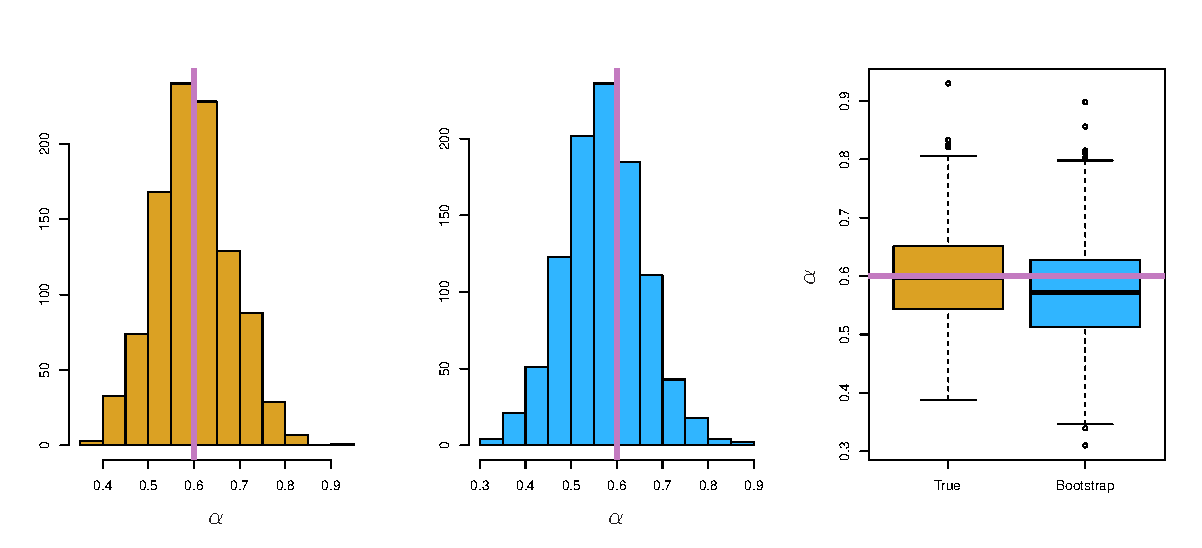
\includegraphics[height=0.4\textheight]{figures/independentVsBootstrap}

\end{figure}

\let\thefootnote\relax\footnotetext{\tiny{Figure 5.10 from \emph{ISLR} (Springer, 2013) with permission from the authors: G. James, D. Witten,  T. Hastie and R. Tibshirani.}}
\end{frame}
%
\begin{frame}{Side note: Bootstrap in Practice}
We can use bootstrap to get error bars in a cheap way.
\begin{itemize}
\item Suppose we have an estimator $\hat{\theta}=\hat{\theta}(\cd_{n})$.

\item To get error bars, we can compute the ``\emph{bootstrap variance}''. 

\begin{itemize}

\item Draw $B$ bootstrap samples.
\item Compute sample variance of $\hat{\theta}(\cd_{n}^{1}),\ldots,\hat{\theta}(\cd_{n}^{B})$..

\item Could report 
\[
\hat{\theta}(\cd_{n})\pm\sqrt{\mbox{Bootstrap Variance}}
\]

\end{itemize}
\end{itemize}
\end{frame}

\begin{frame}
{Ensemble methods}
\onslide<+->{
\begin{simpleblock}
{\textbf{Key ideas:}}
\begin{itemize}
\item \emph{Averaging} i.i.d. estimates reduces variance without making bias worse.
\item Can use bootstrap to simulate multiple data samples.
\end{itemize}
\end{simpleblock}
}
\onslide<+->{
\begin{simpleblock}
{\textbf{Ensemble methods:}}
\begin{itemize}
\item Combine outputs from multiple models.
}
\begin{itemize}[<+->]
\item Same learner on different datasets: ensemble + bootstrap = bagging.
\item Different learners on one dataset: they may make similar errors.
\end{itemize}
\item<+-> Parallel ensemble: models are built independently, \eg bagging
\item<+-> Sequential ensemble: models are built sequentially, \eg boosting
\begin{itemize}[<.->]
\item Try to add new learners that do well where previous learners lack
\end{itemize}
\end{itemize}
\end{simpleblock}
\end{frame}

\subsection{Bagging}
\begin{frame}{Bagging}
\begin{itemize}
\item Draw $B$ bootstrap samples $D^{1},\ldots,D^{B}$ from original data
$\cd$. 

\item Let $\hat{f}_{1},\hat{f}_{2},\ldots,\hat{f}_{B}$ be the prediction
functions from training on $D^{1},\ldots,D^{B}$, respectively.

\pause{}
\item The \textbf{bagged prediction function} is a \emph{combination }of
these:
\[
\hat{f}_{\text{avg}}(x)=\mbox{Combine}\left(\hat{f}_{1}(x),\hat{f}_{2}(x),\ldots,\hat{f}_{B}(x)\right)
\]

\pause{}
\item \dis How might we combine 
\begin{itemize}
\item prediction functions for regression?
\item binary class predictions? 
\item binary probability predictions?
\item multiclass predictions? 
\end{itemize}

\end{itemize}
\end{frame}

\begin{frame}{Out-of-Bag Error Estimation}
\begin{itemize}
\item Each bagged predictor is trained on about 63\% of the data.
\item Remaining 37\% are called \textbf{out-of-bag (OOB)} observations.

\pause{}
\item For $i$th training point, let 
\[
S_{i}=\left\{ b\mid D^{b}\text{ does not contain }i\text{th point}\right\} .
\]

\item The \textbf{OOB prediction} on $x_{i}$ is
\[
\hat{f}_{\text{OOB}}(x_{i})=\frac{1}{\left|S_{i}\right|}\sum_{b\in S_{i}}\hat{f}_{b}(x_{i}).
\]

\item The OOB error is a good estimate of the test error.

\item OOB error is similar to cross validation error -- both are computed
on training set.
\end{itemize}
\end{frame}
%
\begin{frame}{Bagging Classification Trees}
\begin{itemize}
\item Input space $\cx=\reals^{5}$ and output space $\cy=\left\{ -1,1\right\} $.
Sample size $n=30$.
\begin{columns}[t]

\column{.4\textwidth}

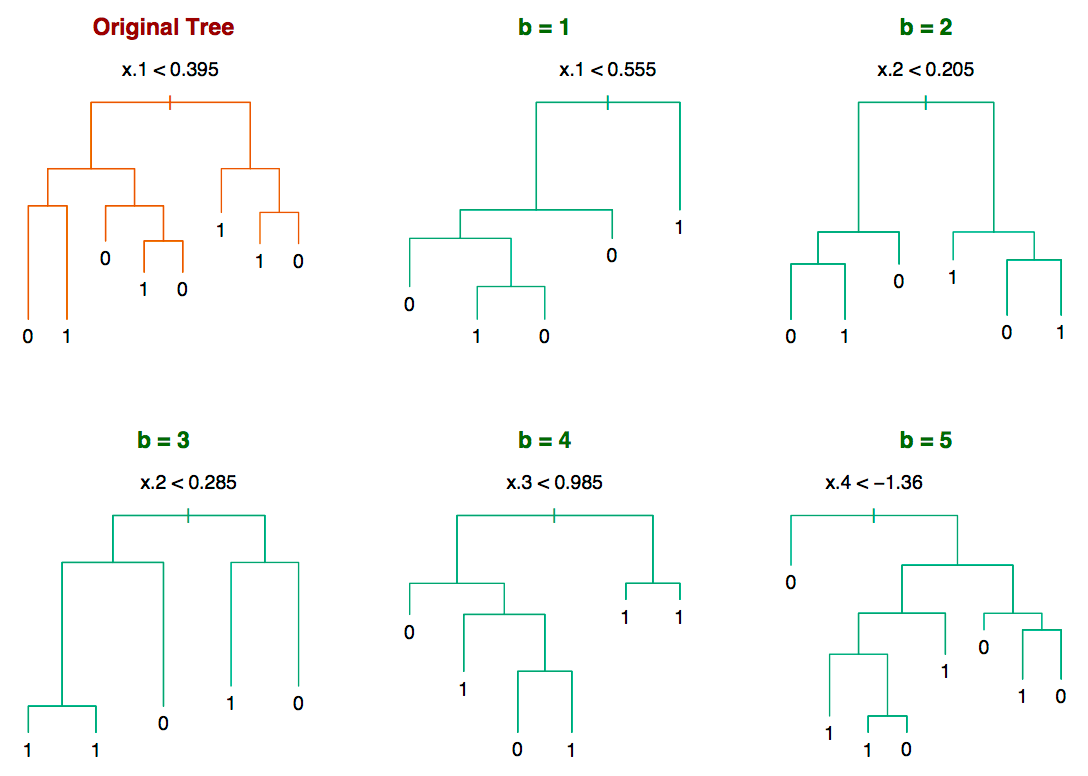
\includegraphics[width=1\columnwidth]{figures/baggedTrees}

\pause{}

\column{.6\textwidth}
\begin{itemize}[<+->]
\item Each bootstrap tree is quite different: different splitting variable at the root

\item \textbf{High variance}: high degree of model variability from small perturbations of the training
data.

\item Conventional wisdom: Bagging helps most when base learners are relatively unbiased but has high variance / low stability $\implies$ decision trees.
\end{itemize}
\end{columns}

\end{itemize}
\let\thefootnote\relax\footnotetext{\tiny{From HTF Figure 8.9}}
\end{frame}
%

\subsection{Random Forests}
\begin{frame}{Variance of a Mean of Correlated Variables}
Recall the motivating principle of bagging:
\begin{itemize}
\item For $\hat{\theta}_{1},\ldots,\hat{\theta}_{n}$ \emph{i.i.d.} with $\ex\pb{\hat{\theta}}=\theta$ and $\var\pb{\hat{\theta}}=\sigma^{2}$,
\[
\ex\left[\frac{1}{n}\sum_{i=1}^{n}\hat{\theta}_{i}\right]=\mu\qquad\var\left[\frac{1}{n}\sum_{i=1}^{n}\hat{\theta}_{i}\right]=\frac{\sigma^{2}}{n}.
\]

\item What if $\hat{\theta}$'s are correlated? 

\pause{}
\item Suppose $\forall i\neq j$, $\text{Corr}(\hat{\theta}_{i},\hat{\theta}_{j})=\rho$ . Then
\[
\var\left[\frac{1}{n}\sum_{i=1}^{n}\hat{\theta}_{i}\right]=\rho\sigma^{2}+\frac{1-\rho}{n}\sigma^{2}.
\]

\item For large $n$, the $\rho\sigma^{2}$ term dominates -- limits benefit
of averaging.
\end{itemize}
\end{frame}

\begin{frame}{Correlation between bootstrap samples}
\begin{itemize}
\item Averaging $\hat{f}_{1},\ldots,\hat{f}_{B}$ reduces variance if they're
based on \emph{i.i.d.} samples from $P_{\cx\times\cy}$

\item Bootstrap samples are 
\begin{itemize}
\item independent samples from the training set, but
\item are \al{not} independent samples from $P_{\cx\times\cy}$.
\end{itemize}

\item This dependence limits the amount of variance reduction we can get.

\pause{}
\item Solution: reduce the dependence between $\hat{f}_{i}$'s by randomization.
\note<.>{How to reduce dependence? Randomization.}
\end{itemize}

\end{frame}
%
\begin{frame}{Random Forest}
\begin{simpleblock}{\textbf{Key idea}}
Use bagged decision trees, but modify the tree-growing procedure
to reduce the dependence between trees.
\end{simpleblock}

\begin{itemize}[<+->]
\item Build a collection of trees independently (in parallel).
\item When constructing each tree node, restrict choice of splitting
variable to a randomly chosen subset of features of size $m$.
\begin{itemize}
\item<.-> Avoid dominance by strong features.
\end{itemize}
\item Typically choose $m\approx\sqrt{p}$, where $p$ is the number of
features.
\item<.-> Can choose $m$ using cross validation.
\end{itemize}
\note[item]{When $m$ is too small, you might underfit. When $m$ is too large, it won't be effective at reducing dependence.}
\end{frame}
%
\begin{frame}{Random Forest: Effect of $m$ size}
\begin{figure}
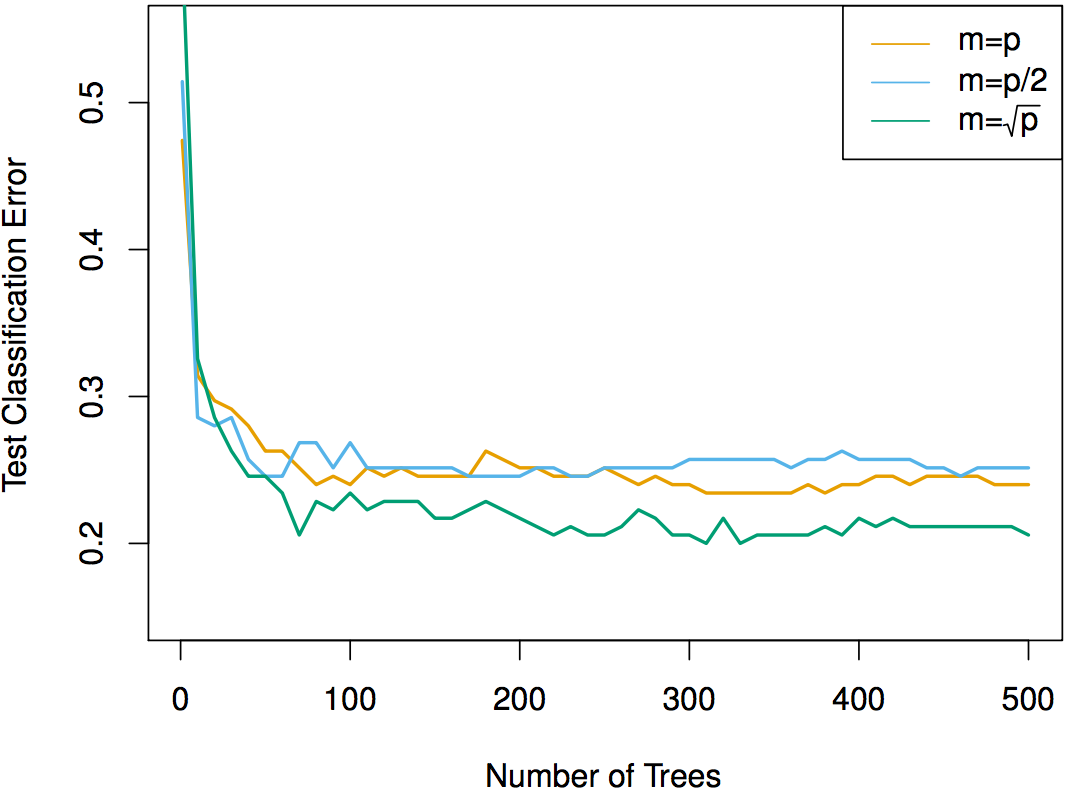
\includegraphics[height=0.7\textheight]{figures/randomForestVsBagging}
\end{figure}

\let\thefootnote\relax\footnotetext{\tiny{From \emph{An Introduction to Statistical Learning, with applications in R} (Springer, 2013) with permission from the authors: G. James, D. Witten,  T. Hastie and R. Tibshirani.}}
\end{frame}

\begin{frame}{Review}
\begin{itemize}[<+->]
\item Usual approach is to build very deep trees---low bias but \al{high variance}
\item Ensembling many models reduces variance
\begin{itemize}[<.->]
\item Motivation: Mean of i.i.d. estimates has smaller variance than single estimate.
\end{itemize}
\item Use bootstrap to simulate many data samples from one dataset
\begin{itemize}[<.->]
\item $\implies$ Bagged decision trees
\end{itemize}
\item But bootstrap samples (and the induced models) are correlated.
\item Bagging seems to work better when we are combining a diverse set of
prediction functions.
\begin{itemize}[<.->]
\item $\implies$ random forests (randomized tree building)
\end{itemize}
\end{itemize}
\end{frame}

\end{document}
